\chapter{Methodology}
\label{chap:met}

The primary objective of this research endeavor is to investigate the process of distilling an LLM into a sequence classification model and to evaluate the efficacy of this methodology compared with alternative approaches. These alternatives include constructing a classifier from the ground up, fine-tuning a pre-trained classifier, and implementing a black-box knowledge distillation technique onto an LLM\@. The efficacy of the models under consideration will be quantitatively assessed based on the accuracy of their predictions on a designated test set.

This chapter details the architecture of the student model and its training process. After that, I provide an elaborate description of the experimental setup, which includes the datasets in use, the architecture of the models under examination, the knowledge distillation techniques employed, and the effectiveness metrics adopted. This systematic exposition aims to provide a clear understanding of the methodologies employed and facilitate a rigorous analysis of their relative merits and demerits in enhancing model performance and efficiency.

\section{Datasets}
\label{sec:datasets}

The datasets selected for this study were specifically chosen for their applicability to the research at hand. The primary criterion for dataset selection is their relevance to classification tasks. Through this targeted dataset selection, the research aims to rigorously evaluate the effectiveness of incorporating rationales into the training process of classification models.

\subsection{Extended Stanford Natural Language Inference (e-SNLI)}
\label{sec:esnli}

To explore the student model's capabilities in classification tasks, we specifically focus on Natural Language Inference (NLI) datasets within the scope of this research. NLI datasets are pivotal for evaluating the model's proficiency in understanding and processing human language. They offer a rich ground for testing its ability to deduce the logical relationship between premises and hypotheses. These datasets consist of sentence pairs annotated with labels indicating whether the hypothesis is true (entailment), false (contradiction), or undetermined (neutral) based on the premise. This dataset was chosen because it is highly suitable for building zero-shot classification pipelines \cite{zeroshotclf}, where the model must accurately categorize data points into classes it has not explicitly been trained on, guided by the nuanced comprehension and application of language and logic facilitated by the LLM knowledge.

Extended Stanford Natural Language Inference (e-SNLI) \cite{esnli} is an extension of the Stanford Natural Language Inference (SNLI) dataset \cite{snli}, which is a widely used benchmark for evaluating NLI models. To create this dataset, annotators were instructed to judge the relation between sentences, given that they describe the same event. Each pair is labeled as ``entailment'', ``neutral'', ``contradiction''. This dataset is particularly useful for evaluating the model's ability to generalize to unseen data and to handle complex and nuanced language constructs.

I have used already generated in \cite{stepbystep} rationales. The authors utilize the Chain-of-Thought (CoT) \cite{cot} prompting approach to instruct LLM on generating rationales. This method involves creating a prompt template containing triplets of example inputs, corresponding labels, and user-provided rationales explaining the reasoning behind each association. By appending each dataset input to this template and using it to prompt the PaLM 540B LLM \cite{palm}, the authors guide the model to produce both rationales and labels for each input. This process enables the LLM to replicate the demonstrated reasoning in the template, generating coherent rationales that explain the logic leading to its predictions. The example of the collected data is depicted in Fig. \ref{fig:rationale_dataset}.

\begin{figure}[hbt]
    \centering
    \begin{subfigure}[t]{.5\linewidth}
        \centering
        \lstinputlisting[breaklines=true,breakatwhitespace,breakindent=0em,basicstyle=\footnotesize]{figs/data_example_1.txt}
    \end{subfigure}%
    \begin{subfigure}[t]{.5\linewidth}
        \centering
        \lstinputlisting[breaklines=true,breakatwhitespace,breakindent=0em,basicstyle=\footnotesize]{figs/data_example_2.txt}
    \end{subfigure}

    \caption{Data examples from the e-SNLI dataset, refined with rationale.}
    \label{fig:rationale_dataset}
\end{figure}

The dataset initially comprised 569,033 samples, each annotated with an original label, an LLM-predicted label, and an LLM-provided rationale. For specific reasons related to ensuring consistency and reliability in training and evaluation, I excluded samples whose original label did not align with the LLM prediction label. This curation process resulted in a refined dataset consisting of 399,566 samples. The resulting dataset is available at \linebreak \url{https://hf.co/datasets/batalovme/esnli_with_rationale}.

To conserve computational resources and ensure simplicity in analysis, this study will strategically utilize only $10\%$ of the available dataset. This approach not only facilitates more efficient data processing but also aligns with the objectives of managing system load and expediting analytical outcomes.

\subsection{Web Of Science (WOS-11967)}
\label{sec:wos}

For a classic multi-class classification task, I selected the WOS-11967 dataset \cite{wos}, which comprises 11,967 documents distributed across 35 categories. By focusing solely on these parent categories, the dataset provides an excellent foundation for evaluating the model's performance in classifying documents into discrete categories. This choice is particularly advantageous because the dataset encompasses a diverse array of topics, presenting a significant challenge to the model's ability to accurately discern and categorize complex and varied content. The distribution of the classes within the dataset is illustrated in \autoref{fig:wos_distrib}.

\begin{figure}[hbt]
    \centering
    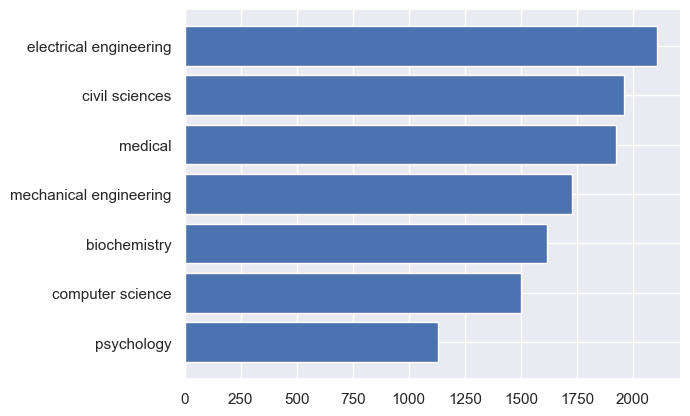
\includegraphics[width=0.8\linewidth]{figs/wos_distrib.png}
    \caption{The class distribution of the sample of the WOS-11967 dataset}
    \label{fig:wos_distrib}
\end{figure}

To conserve resources typically expended on extracting rationales from LLM, I strategically extracted a subset of 4,787 samples from the dataset, maintaining the same class distribution as the original. This method not only streamlines the computational demands but also allows for a more focused examination of the model's capability to handle and classify data effectively under a substantially reduced dataset size.

For the generation of rationales within the dataset, I employed a methodology similar to the one used for the e-SNLI dataset, focusing initially on creating two example rationales for each category for few-shot learning with the LLM\@. These rationales were generated by prompting GPT-3.5 using prompt depicted at \autoref{fig:wos_eg_prompt}.

\begin{figure}[ht!]
    \centering
    \lstinputlisting[columns=fullflexible,basicstyle=\small,breaklines=true,breakatwhitespace,breakindent=0em,xleftmargin=1.5cm,xrightmargin=1.5cm,backgroundcolor=\color{lightgray},frame=tlbr,framesep=0.5cm,framerule=0pt]{figs/wos_example_prompt.txt}
    \caption{Prompt for generating example rationales (for few-shot prompting) for the WOS-11967 dataset.}
    \label{fig:wos_eg_prompt}
\end{figure}

After collecting these samples for few-shot learning, I conducted a thorough manual review of each entry. This step was crucial to ensuring the quality and consistency of the example shots for the LLM\@.

Using these curated example rationales, I engaged GPT-3.5 in a few-shot learning scenario, where the model was fed with the examples along the prompt to generate rationales.

\begin{figure}[ht!]
    \centering
    \lstinputlisting[columns=fullflexible,basicstyle=\small,breaklines=true,breakatwhitespace,breakindent=0em,xleftmargin=1.5cm,xrightmargin=1.5cm,backgroundcolor=\color{lightgray},frame=tlbr,framesep=0.5cm,framerule=0pt]{figs/wos_prompt.txt}
    \caption{Prompt for generating rationales for the WOS-11967 dataset.}
    \label{fig:wos_prompt}
\end{figure}

This rigorous process ensures that the rationales are not only generated efficiently but also of high quality and consistency, thereby enhancing the dataset's reliability for subsequent ML tasks.

The resulting dataset consists of 4,787 samples, each annotated with an original label and an LLM-provided rationale. The dataset is available at \linebreak \url{https://hf.co/datasets/batalovme/wos_with_rationale}.

\section{Baseline models and methods}
\label{sec:baselines}

In evaluating sequence classification methodologies, robust baseline models for comparison are imperative. These models serve as a benchmark against which the efficacy of the distillation process from LLMs to sequence classification models can be measured. This section comprehensively describes the baseline models considered in this study and their results on the datasets under examination.

\subsection{RoBERTa (Robustly Optimized BERT Approach)}

Developed by \citeauthor{roberta} \cite{roberta}, RoBERTa is an enhanced version of BERT (Bidirectional Encoder Representations from Transformers) \cite{bert}, optimized for more robust performance in natural language processing (NLP) tasks.

RoBERTa utilizes a specialized structure within the Transformer's encoder architecture for sequence classification tasks. Instead of employing a separate decoder, the model leverages the output of a special classification token, commonly known as the CLS token, which is added at the beginning of every input sequence. During pre-training, RoBERTa learns to embed a rich representation of the entire input sequence into this CLS token. This representation is typically passed through a simple feed-forward network to produce the probability distribution over the possible classes.

\subsection{T5 (Text-to-Text Transfer Transformer)}

Introduced by \citeauthor{t5} \cite{t5}, T5 redefines the approach to NLP tasks by treating every task as a text-to-text problem. This model simplifies the application of transfer learning by using a unified framework across different tasks, including sequence classification.

T5's architecture is based on the Transformer model, which consists of an encoder-decoder structure. The encoder processes the input text while the decoder generates the output text. In the context of sequence classification, the model is trained to predict the class label based on the input text. This process involves encoding and decoding the input text to generate the class label as a text.

\subsection{EncT5}

The second variant of the T5 model -- EncT5, which only utilizes the pre-trained encoder part \cite{enct5}. This variant is particularly well-suited for sequence classification tasks, as it focuses solely on the input text and does not require generating output text. This model configuration, which avoids the generative complexities of the decoder, utilizes a single `0 token logits' mechanism where a precisely mapped embedding of this token is learned during training to pool information effectively from the entire encoder output. By focusing solely on the encoder and optimizing the information pooling process, EncT5 achieves computational efficiency and simplifies the model architecture.

\subsection{Distilling Step-by-Step!}

Another variant of the T5 model is the methodological framework developed by \citeauthor{stepbystep} \cite{stepbystep}. In their approach, the authors employ LLM rationales as a supplementary source of supervision during the training of smaller, task-specific models within a comprehensive multi-task learning framework.

The first task is dedicated to generating labels that are direct annotations corresponding to the data instances, facilitating a straightforward supervised learning process. The second task involves the generation of rationales, which are explanatory texts that elucidate the reasoning behind the labels provided by the model. This rationales generation task prefix not only augments the transparency of the model's decisions but also provides additional contextual data that aids in refining the training of the Seq2Seq student models.

The model employs only the task prefix associated with label generation at the inference stage. This strategic focus ensures that the output is streamlined for practical application, omitting the rationale generation process to enhance efficiency and response time in real-world operational settings. Such an approach underscores the model's adaptability and potential for application in scenarios where quick decision-making is paramount. An overview of this methodology is illustrated in \autoref{fig:stepbystep}.

\begin{figure}[hbt]
    \centering
    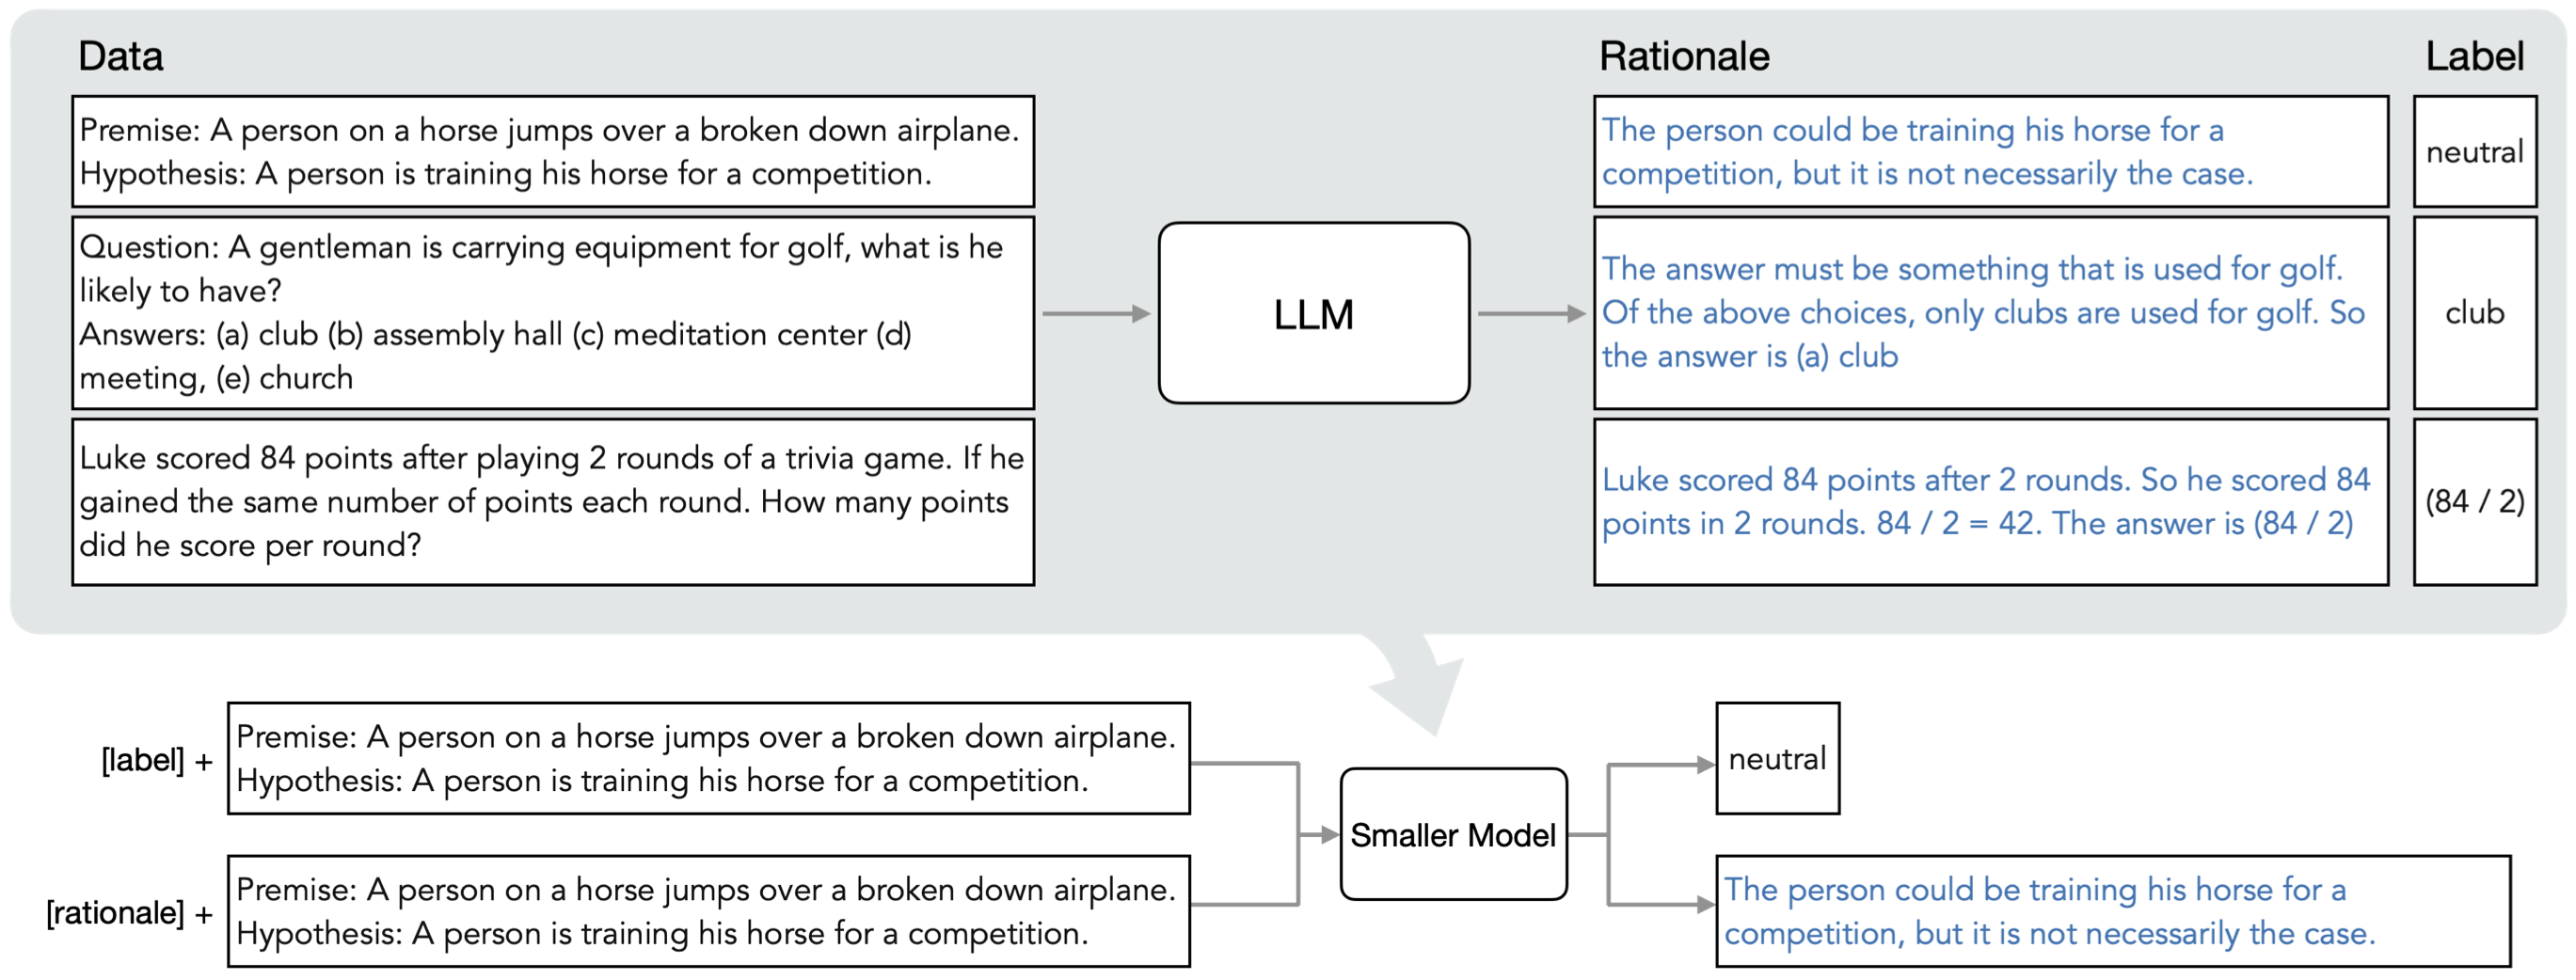
\includegraphics[width=0.99\linewidth]{figs/stepbystep.png}
    \caption[Overview on Distilling step-by-step method.]{Overview on Distilling step-by-step method. Source: \cite{stepbystep}.}
    \label{fig:stepbystep}
\end{figure}

\autoref{tab:baseline_models} presents a comparative summary of baseline models for evaluating the performance metrics. This table categorizes each model based on its setup and number of parameters and provides a shorthand notation for reference. The "Model" column lists the model name from HuggingFace Hub\footnote{\url{https://hf.co/models}}.

\begin{table}[h]
    \centering
    \caption{Baseline Models}
    \label{tab:baseline_models}
    \resizebox{\textwidth}{!}{
        \begin{tabular}{llcr}
            \toprule
            \textbf{Model}                                                          & \textbf{Setup}           & \textbf{Parameters} & \textbf{Short Name}    \\
            \midrule
            \href{https://hf.co/FacebookAI/roberta-base}{FacebookAI/roberta-base}   & Seq. Classification      & 125M\footnotemark   & RoBERTa Base           \\
            \href{https://hf.co/FacebookAI/roberta-large}{FacebookAI/roberta-large} & Seq. Classification      & 355M                & RoBERTa Large          \\
            \href{https://hf.co/google-t5/t5-base}{google-t5/t5-base}               & Seq2Seq                  & 223M                & T5 Base (Seq2Seq)      \\
            \href{https://hf.co/google-t5/t5-base}{google-t5/t5-base}               & Seq. Classification      & 109M                & EncT5 Base             \\
            \href{https://hf.co/google-t5/t5-base}{google-t5/t5-base}               & Distilling Step-by-Step! & 223M                & T5 Base (Step-by-Step) \\
            \bottomrule
        \end{tabular}}
\end{table}

\footnotetext{M herinafter means millions of parameters}

\section{Metrics for evaluation}
\label{sec:metrics}

The evaluation of classification models on the provided datasets necessitates a comprehensive analysis using standard performance metrics. To accurately gauge the effectiveness of models deployed on these datasets, we employ a suite of metrics: accuracy, precision, recall, and F1 score.

Each metric provides unique insights into different aspects of the model's performance, thus facilitating a robust assessment of its capabilities in handling text classification tasks.

\subsection{Accuracy}

Accuracy is the most commonly used metric for evaluating performance in classification tasks. Accuracy represents the proportion of total predictions that the model classified correctly. It is calculated as the ratio of correctly predicted observations:
$$
    \text{Accuracy} = \frac{\text{Number of Correct Predictions}}{\text{Total Number of Input Data}}
$$

This metric is particularly straightforward and provides an immediate understanding of the overall effectiveness of the model. Fortunately, the same metric used in binary classification can be applied to multi-class classification problems without modification.

However, it may not always be the most reliable metric in datasets with imbalanced classes. In scenarios characterized by class imbalance, reliance on accuracy as a metric can be deceptive. It often presents an inflated score despite the model's inadequate performance in predicting minority classes. For instance, consider an evaluation set with eight instances of class 0 and two instances of class 1. If a model consistently predicts class 0 for all inputs, it would achieve an accuracy of $80\%$. However, this does not signify a well-performing model, as it fails to identify any instances of the minority class.

To gain a more comprehensive understanding of a classifier's performance in situations of class imbalance, it is advisable to examine metrics such as precision and recall. These metrics offer a more nuanced insight into the classifier's error dynamics across different classes, thereby revealing its effectiveness in correctly identifying each class.

\subsection{Understanding True Positives, False Positives, True Negatives, and False Negatives}

To facilitate a deeper understanding of the other metrics discussed, it is imperative to define the core components that constitute these measurements: True Positives (TP), False Positives (FP), True Negatives (TN), and False Negatives (FN). These terms are foundational in constructing the confusion matrix, a tool used to visualize the performance of a binary classification model. Below, I present a \autoref{tab:confusion_matrix} that elucidates these components.

\begin{table}[h]
    \centering
    \caption{Confusion Matrix}
    \begin{tabular}{|c|c|c|}
        \hline
                                          & \multicolumn{2}{c|}{\textbf{Predicted}}                       \\ \cline{2-3}
        \multirow{-2}{*}{\textbf{Actual}} & Positive                                & Negative            \\
        \hline
        Positive                          & True Positive (TP)                      & False Negative (FN) \\
        \hline
        Negative                          & False Positive (FP)                     & True Negative (TN)  \\
        \hline
    \end{tabular}

    \label{tab:confusion_matrix}
\end{table}


\subsection{Precision}

Precision, or positive predictive value, measures the accuracy of the positive predictions made by the model. It is defined as the ratio of true positive predictions to the total predicted positives:

$$
    \text{Precision} = \frac{\text{True Positives}}{\text{True Positives} + \text{False Positives}}
$$

Essentially, precision evaluates the model's ability to correctly identify instances of a specific class. This metric is essential in situations where the consequences of a false positive are significant, such as in document classification tasks within the WOS (\autoref{sec:wos}). High precision is crucial for ensuring documents are accurately categorized, minimizing misclassification risk.

\subsection{Recall}

Recall, also known as sensitivity or true positive rate, quantifies the model's ability to identify all relevant instances within a dataset. It is calculated as follows:

$$
    \text{Recall} = \frac{\text{True Positives}}{\text{True Positives} + \text{False Negatives}}
$$

In simpler terms, recall evaluates the model's capability to detect every instance of a specific class. High recall is crucial in critical applications where missing true positives could lead to dire outcomes. For example, in the e-SNLI dataset (\autoref{sec:esnli}), achieving high recall implies that the model effectively recognizes the majority of accurate entailments, contradictions, or neutral statements based on the provided premises.

The most detailed and intuitive explanation of the metrics precision and recall is provided at the \autoref{fig:precisionrecall}.

\begin{figure}[h!]
    \centering
    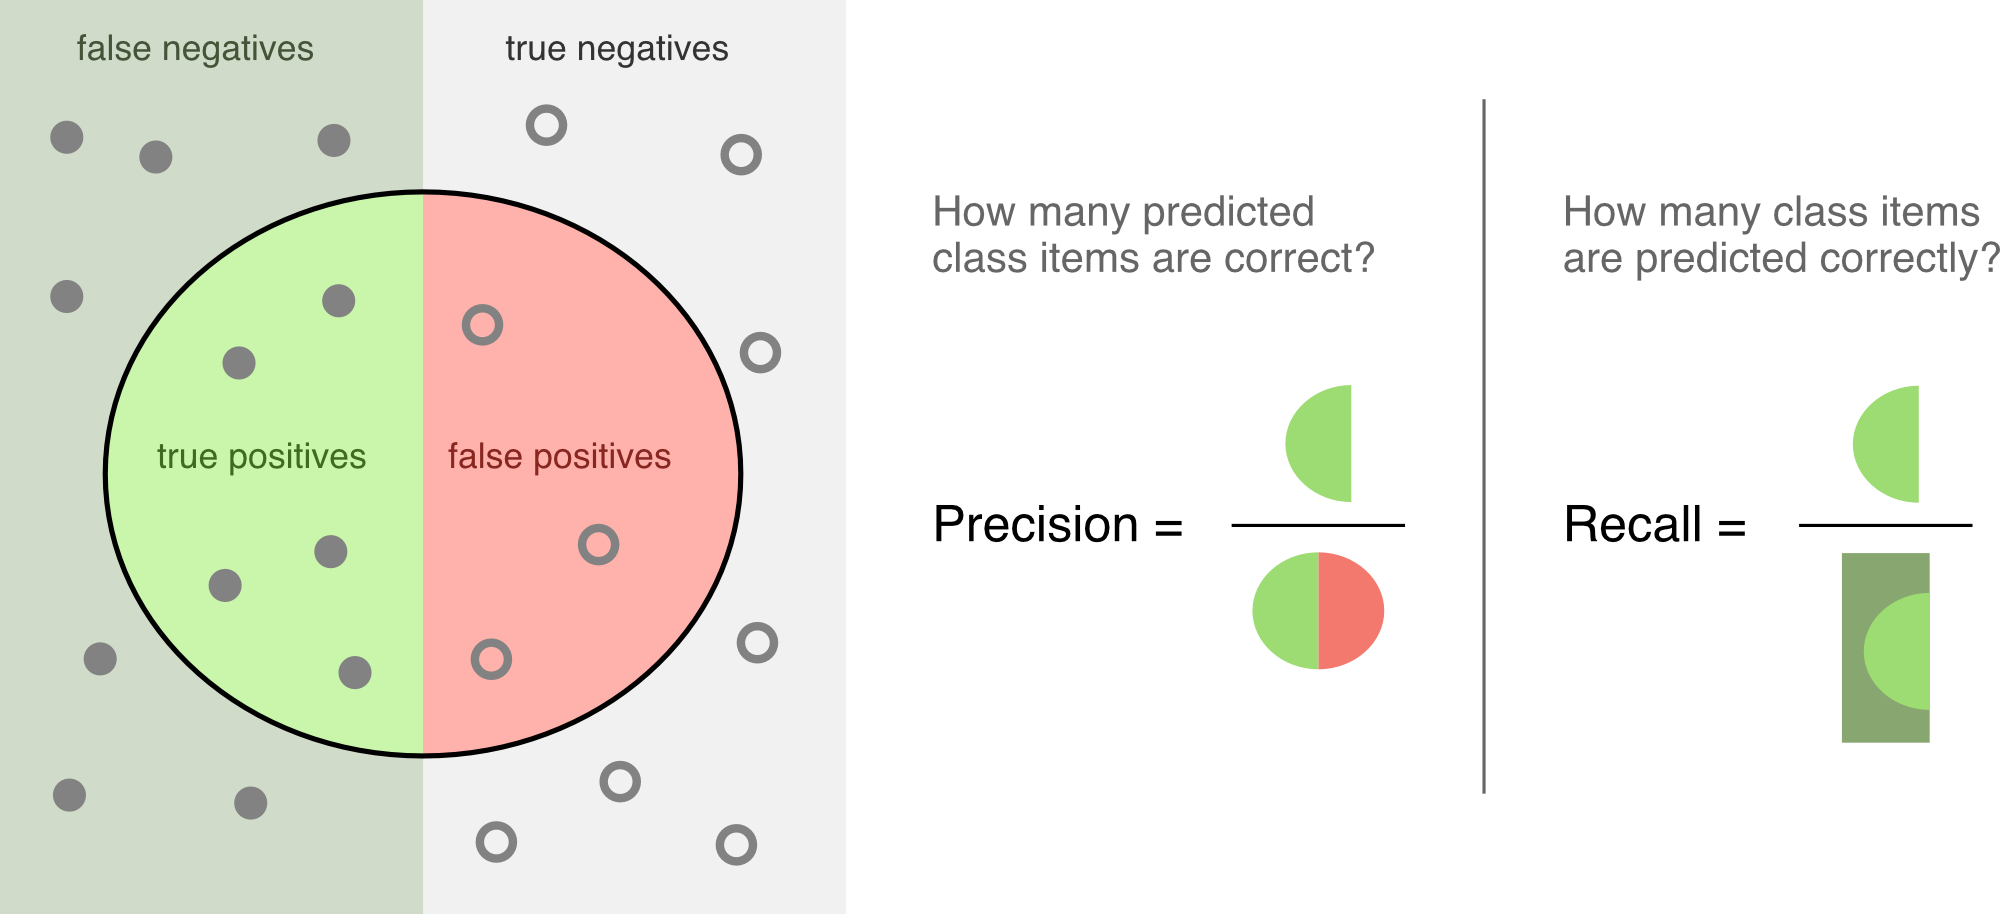
\includegraphics[width=0.9\linewidth]{figs/precisionrecall.jpg}
    \caption[Precision and recall]{Precision and recall. Adopted from Wikipedia\protect\footnotemark.}
    \label{fig:precisionrecall}
\end{figure}


\subsection{F1 Score}
The F1 score is the harmonic mean of precision and recall, providing a balance between the two by taking both false positives and false negatives into account:

$$
    \text{F1 Score} = 2 \times \frac{\text{Precision} \times \text{Recall}}{\text{Precision} + \text{Recall}}
$$

This metric is beneficial when there is an uneven class distribution, as is common in many real-world datasets, including those in NLP tasks like used in this study. The F1 score is a single measure to capture both aspects of model accuracy concerning positive class predictions.

\footnotetext{Source available at \url{https://en.wikipedia.org/wiki/Precision_and_recall}}

\section{Proposed knowlegde distillation method}
\label{sec:proposed_method}

In this study, the primary focus is on black-box distillation methods (refer to \autoref{section:blackbox}). These methods rely exclusively on the output predictions of teacher models, enabling the utilization of any non-open-source LLM as a teacher. This approach is particularly advantageous as it does not require access to the internal architecture or weights of the LLM, thereby circumventing potential intellectual property and accessibility issues.

During the experiments (Sections \ref{sec:t5_2heads} - \ref{sec:roberta_rationales}), several methods for distilling knowledge from LLM into sequence classification models were described and evaluated. This section describes the most successful method identified through these experimental trials.

\subsection*{Method Overview}

The proposed method consists of a two-part pipeline:
\begin{itemize}
    \item \textbf{Rationale Generation with T5:} The T5 Seq2Seq model is employed to generate rationales. It is specifically trained on a dataset of text inputs paired with rationales generated by LLM, focusing on capturing the LLM's reasoning process.
    \item \textbf{Classification with RoBERTa:} Following rationale generation, a RoBERTa model is used to perform the final classification. RoBERTa, classifies the input and the generated by T5 rationales rather than the raw text.
\end{itemize}

\subsection*{Training Procedure}

The training procedure for the pipeline begins with preparing the T5 model to generate rationales. This involves creating a dataset part where each entry consists of an input and a corresponding rationale. The T5 model is then fine-tuned on this dataset, learning to mimic LLM in generating rationales that explain or contextualize the inputs provided.

Once the T5 model is adequately trained, it is used to generate rationales for a new dataset. These generated rationales were added to the training dataset for the classification with their original inputs and labels. This new dataset serves as the training data for the RoBERTa or another classification model.

In the next step, the RoBERTa model is fine-tuned on the input-rationale pairs to classify the label based on the rationales generated by the T5 model. Through this process, RoBERTa learns to make predictions that are informed by the context provided in the rationales.

The training pipeline of the proposed method is visualized in \autoref{fig:pipeline_training}.

\begin{figure}[hbt]
    \centering
    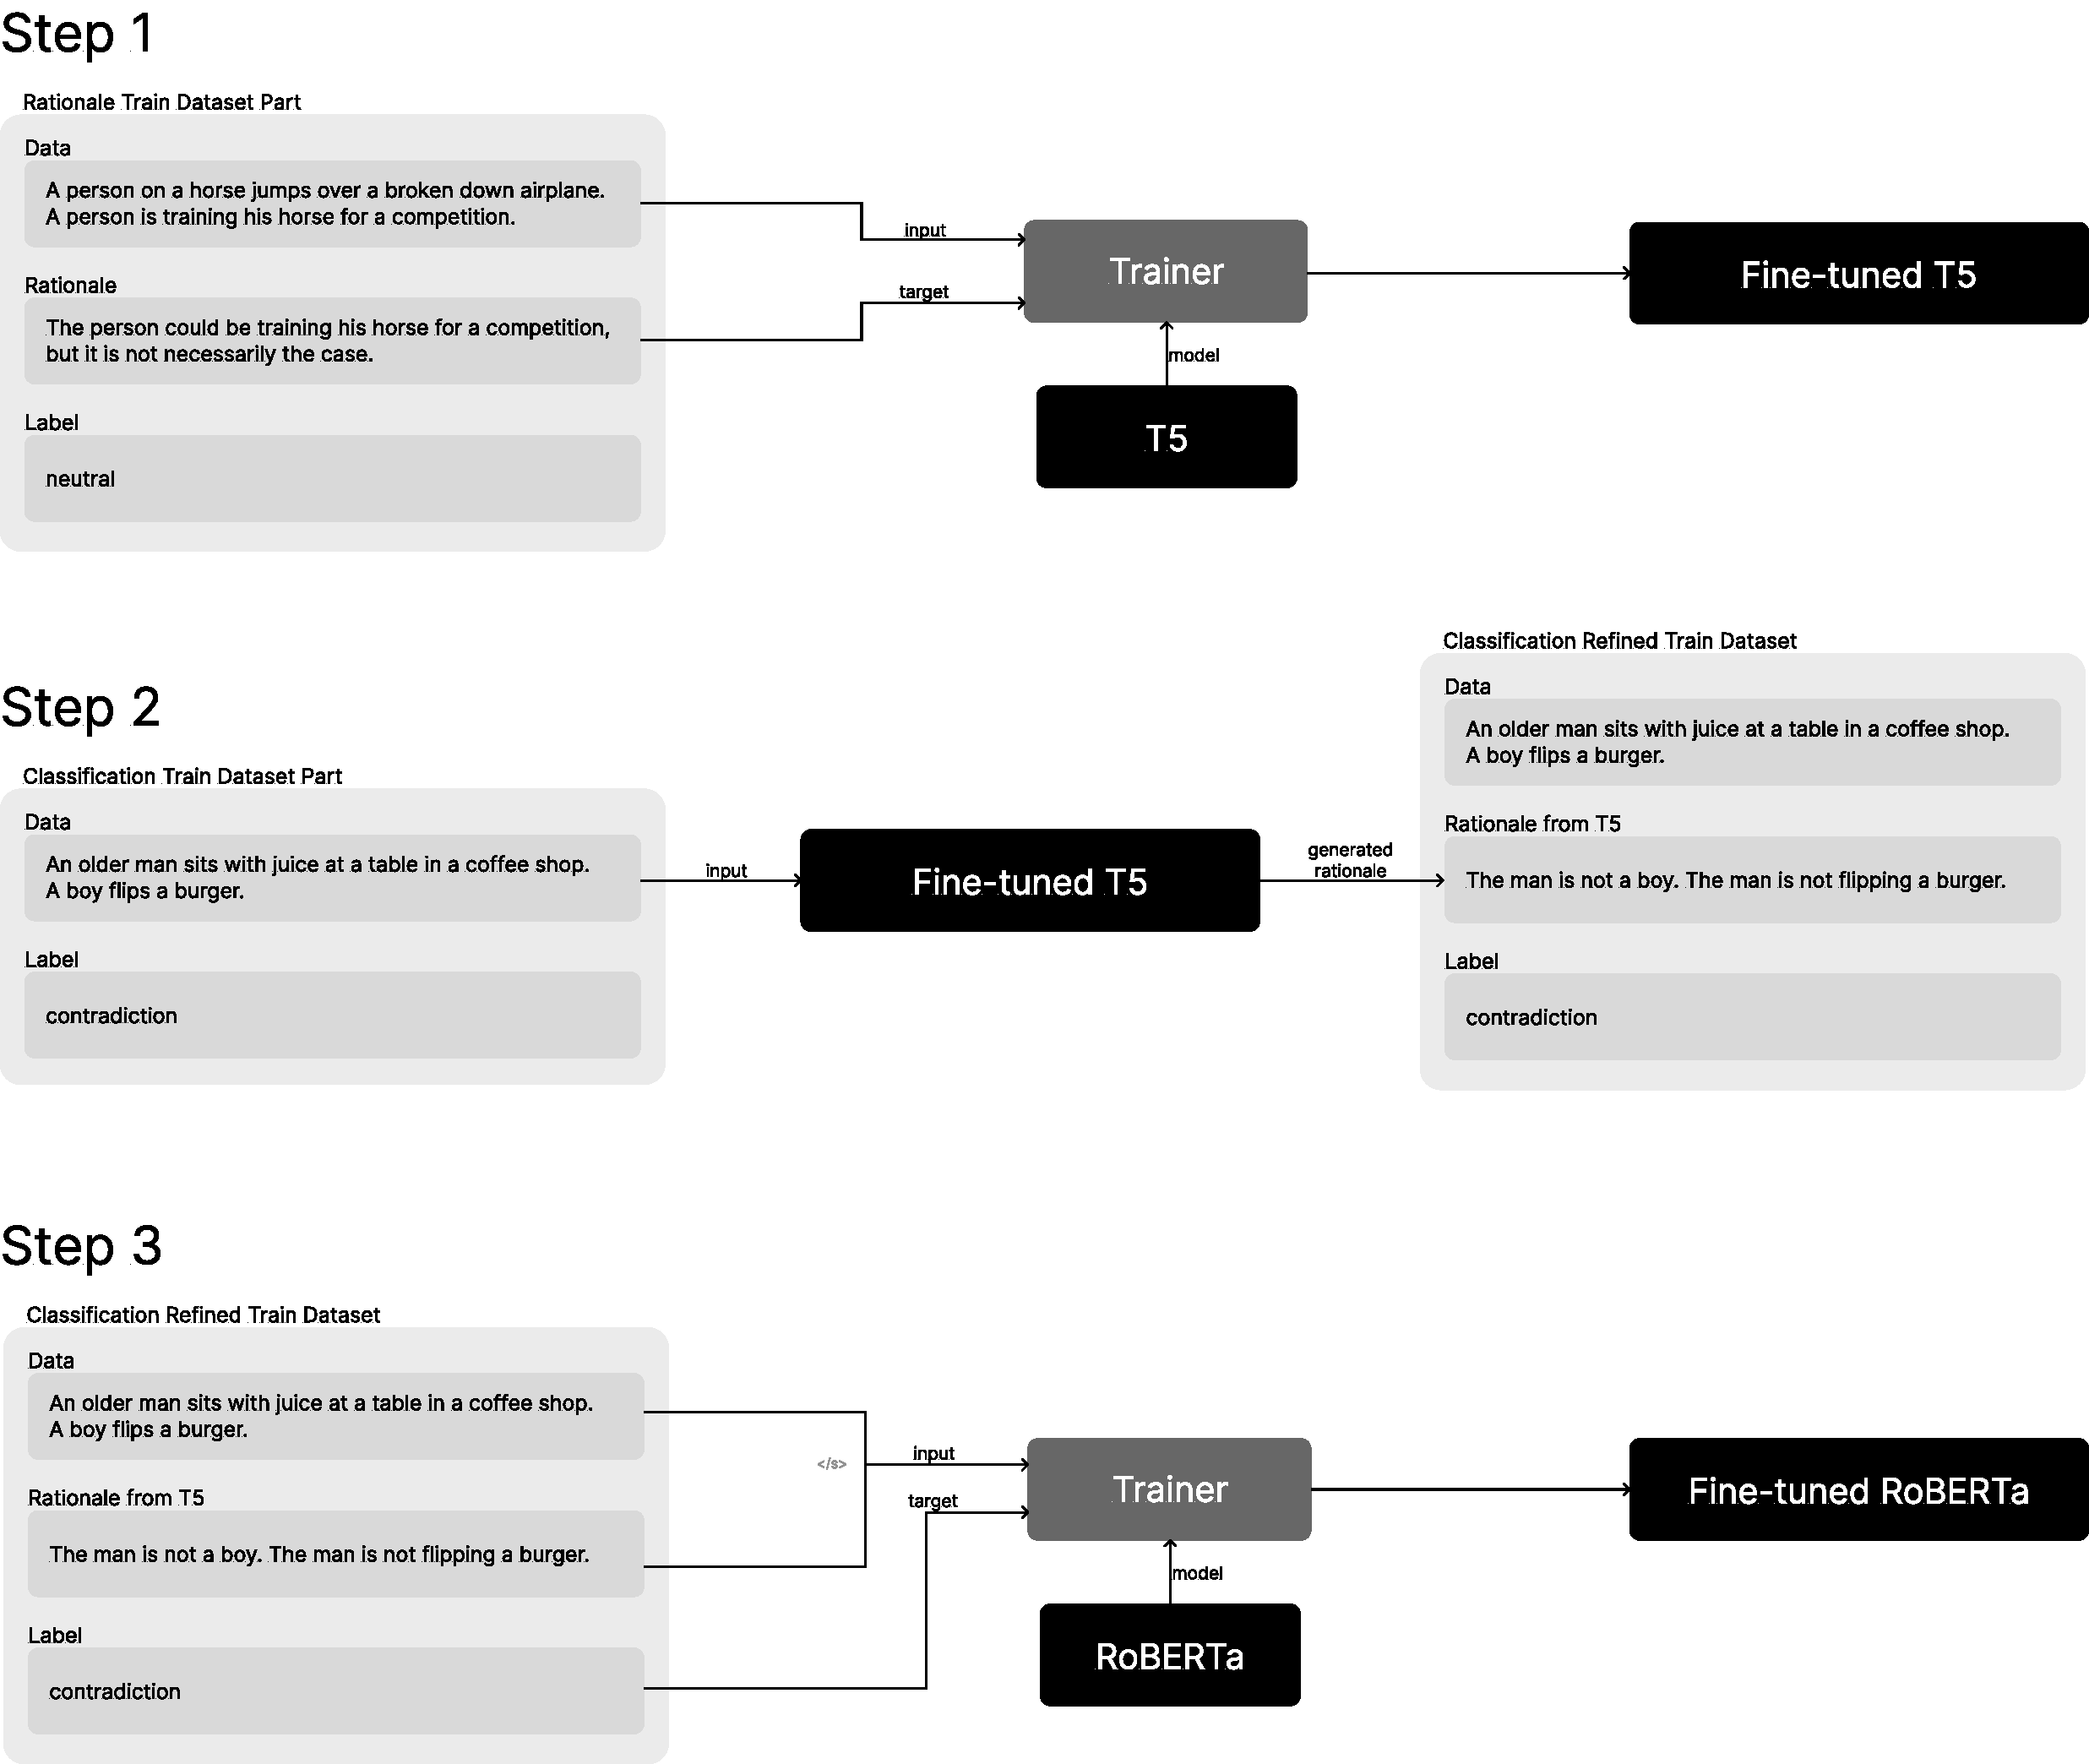
\includegraphics[width=\linewidth]{figs/pipeline_training.pdf}
    \caption{Training procedure of the proposed method.}
    \label{fig:pipeline_training}
\end{figure}

\subsection*{Inferece Procedure}

During inference, the T5 model first processes new, unseen inputs to generate rationales. Then, input-rationales pairs are fed into the RoBERTa model, which is used to classify the label.

This dual-model approach leverages the generative capabilities of the T5 model to create interpretable rationales, which are then used by the RoBERTa model to make classifications. This method not only enhances the accuracy by focusing on the most relevant aspects of the text through the rationales but also aims to improve the interpretability of the model's decisions. This structured training and inference framework allows for the effective utilization of complex language understanding in a more resource-efficient manner.
